\chapter{Tidal Energy Assignment 2}
\label{ch:tidal}

% Structure follows Tidal_energy_assignment_2026.pdf.
% Group 21 data verified against Appendix 1 and pre-assignment slide 4:
% Adm. Ref.: SN167BV; latitude: 47 33.7N; longitude: 02 54.9W
% (Appendix 1 only lists groups 1-20, so group 21 wraps around to row 1).
% Peak spring current: 5.2 knots; peak neap current: 3.5 knots; FZU: 0.
% Constituent amplitudes [m/s]: M2 = 2.2185; S2 = 0.4335; K2 = 0.4437.
% Constituent periods [hours], pre-assignment slides 5--6:
% M2 = 12.4206; S2 = 12.0; K2 = 11.965.
% All numerical results below were produced with the notebooks and the
% tidaltools package in assignment2/ of the companion repository, and are
% reproduced here for the write-up.

\section{Environmental Data and Tidal Resource}
\label{sec:tidal-resource}

\subsection{Site and Environmental Data}
\label{sec:tidal-site}
The assigned site is SN167BV, located at
$47^\circ 33.7'\mathrm{N}$, $02^\circ 54.9'\mathrm{W}$.
Table~\ref{tab:tidal-site} presents the supplied tidal data
for this site. The Formzahl number is zero, indicating
a semi-diurnal tidal regime.

\begin{table}[H]
    \centering
    \caption{Supplied tidal data for site SN167BV.}
    \label{tab:tidal-site}
    \small
    \setlength{\tabcolsep}{4pt}
    \begin{tabular}{lcccccccc}
        \hline
        Adm. Ref. & Lat. & Long. & Pk Sp & Pk Np & FZU
        & M2 & S2 & K2 \\
        & & & [kt] & [kt] & [-]
        & [m/s] & [m/s] & [m/s] \\
        \hline
        SN167BV & $47^\circ 33.7'\mathrm{N}$
        & $02^\circ 54.9'\mathrm{W}$
        & 5.2 & 3.5 & 0 & 2.2185 & 0.4335 & 0.4437 \\
        \hline
    \end{tabular}
\end{table}


\subsection{Harmonic Reconstruction of the Tidal Current}
\label{sec:tidal-harmonics}
The tidal current velocity was calculated by summing the contributions of the three constituents:

\begin{equation}
    U(t) = \sum_{i=1}^{3} U_{A,i}
    \cos\left(\frac{2\pi t}{T_{A,i}}+\varphi_i\right).
    \label{eq:tidal-current}
\end{equation}

Since no phase information was provided, all phases were set to zero, so the constituents align at the start. Current velocities were calculated hourly for one year, giving 8,760 values. Positive and negative values indicate opposite flow directions.

As a check, the reconstructed series was compared against the tabulated peak spring and neap currents. The sum $M2+S2 = 2.652\,\mathrm{m/s}$ and the difference $M2-S2 = 1.785\,\mathrm{m/s}$ closely reproduce the tabulated peak spring ($5.2\,\mathrm{kt} = 2.675\,\mathrm{m/s}$) and peak neap ($3.5\,\mathrm{kt}=1.801\,\mathrm{m/s}$) currents, confirming the constituent data and periods are consistent with each other.

\subsection{Spring-Neap Cycle}
\label{sec:tidal-cycle}
\begin{figure}[H]
    \centering
    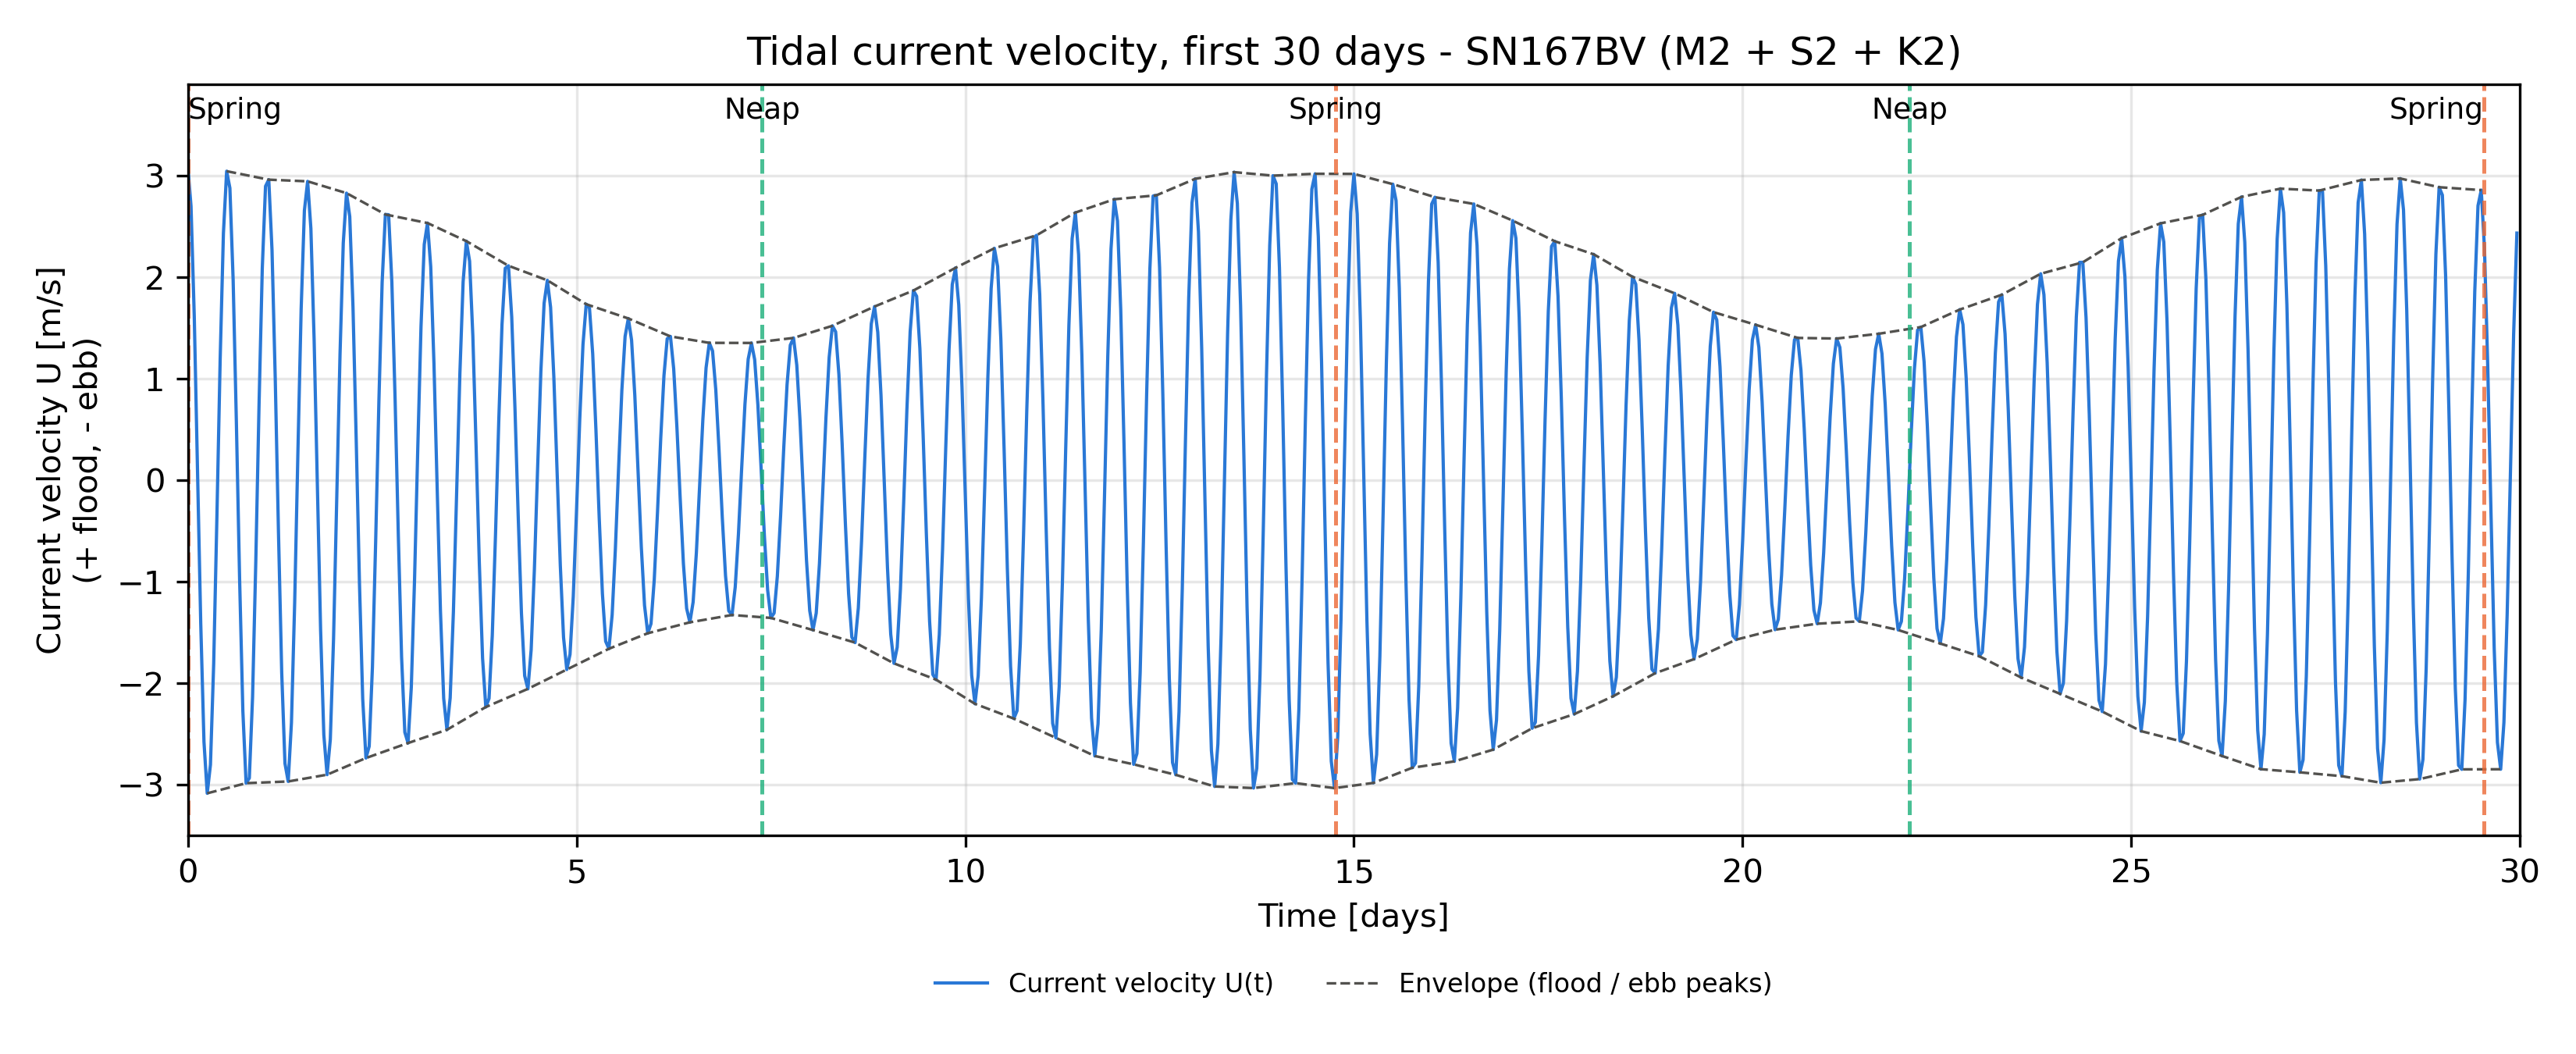
\includegraphics[width=\textwidth]
    {figures/tidal/part1_tidal_velocity_30days.png}
    \caption{Reconstructed tidal current velocity over
    the first 30 days, showing the spring-neap cycle.}
    \label{fig:tidal-current}
\end{figure}
Figure~\ref{fig:tidal-current} shows the repeated changes in current direction and the changing peak velocities over the spring-neap cycle. During spring tides, the constituents reinforce each other, producing stronger currents. During neap tides, they partially cancel each other, producing weaker currents.
The beat between the M2 and S2 constituents sets the spring-neap period,

\begin{equation}
    T_{sn} = \left(\frac{1}{T_{S2}} - \frac{1}{T_{M2}}\right)^{-1},
    \label{eq:tidal-beat}
\end{equation}

which evaluates to $T_{sn} = 354.4\,\mathrm{h} = 14.77$ days. Spring tides occur approximately around days 0, 15 and 30, with neap tides around days 7 and 22. These timings are approximate because K2 also influences the peaks. Figure 1.1 therefore shows approximately two spring-neap cycles.

Because K2 beats slowly against S2 (period of order half a year), the peak spring current is not constant through the year: at the strongest springs it reaches approximately $3.10\,\mathrm{m/s}$, slightly above the $3.0\,\mathrm{m/s}$ cut-out speed of the turbine used in Section~\ref{sec:tidal-stream}. The mean current speed over the full year is $1.44\,\mathrm{m/s}$.

\section{Tidal Stream Energy Production}
\label{sec:tidal-stream}

\subsection{Turbine Characteristics and Power Curve}
\label{sec:stream-turbine}
The reconstructed current from Section~\ref{sec:tidal-resource} drives a bi-directional hydrokinetic turbine with the characteristics listed in Table~\ref{tab:stream-turbine}.

\begin{table}[H]
    \centering
    \caption{Bi-directional hydrokinetic turbine characteristics.}
    \label{tab:stream-turbine}
    \begin{tabular}{lc}
        \hline
        Quantity & Value \\
        \hline
        Cut-in speed & $1.0\,\mathrm{m/s}$ \\
        Cut-out speed & $3.0\,\mathrm{m/s}$ \\
        Rated power & $1.0\,\mathrm{MWe}$ \\
        Total efficiency (water to electricity) & $0.45$ \\
        Capture area & $165\,\mathrm{m^2}$ \\
        Water density $\rho_{water}$ & $1025\,\mathrm{kg/m^3}$ \\
        \hline
    \end{tabular}
\end{table}

Because the turbine is bi-directional it produces the same power on flood and ebb, so only the current magnitude $|U|$ determines the output. The electrical power is given by

\begin{equation}
    P(U) =
    \begin{cases}
        0 & |U| < U_{ci} \\
        \min\left(\tfrac{1}{2}\rho A \eta |U|^3,\ P_{rated}\right) & U_{ci} \le |U| \le U_{co} \\
        0 & |U| > U_{co}
    \end{cases}
    \label{eq:stream-power}
\end{equation}

Equating the cubic term to the rated power gives the rated current speed,

\begin{equation}
    U_{r} = \left(\frac{P_{rated}}{\tfrac{1}{2}\rho A \eta}\right)^{1/3},
    \label{eq:stream-rated}
\end{equation}

which evaluates to $U_r = 2.973\,\mathrm{m/s}$, only marginally below the $3.0\,\mathrm{m/s}$ cut-out. Consequently the turbine has almost no flat, rated-power plateau: it follows the cubic law up to approximately $1\,\mathrm{MW}$ and then shuts down shortly afterwards. The resulting power curve is shown in Figure~\ref{fig:stream-power-curve}.

\begin{figure}[H]
    \centering
    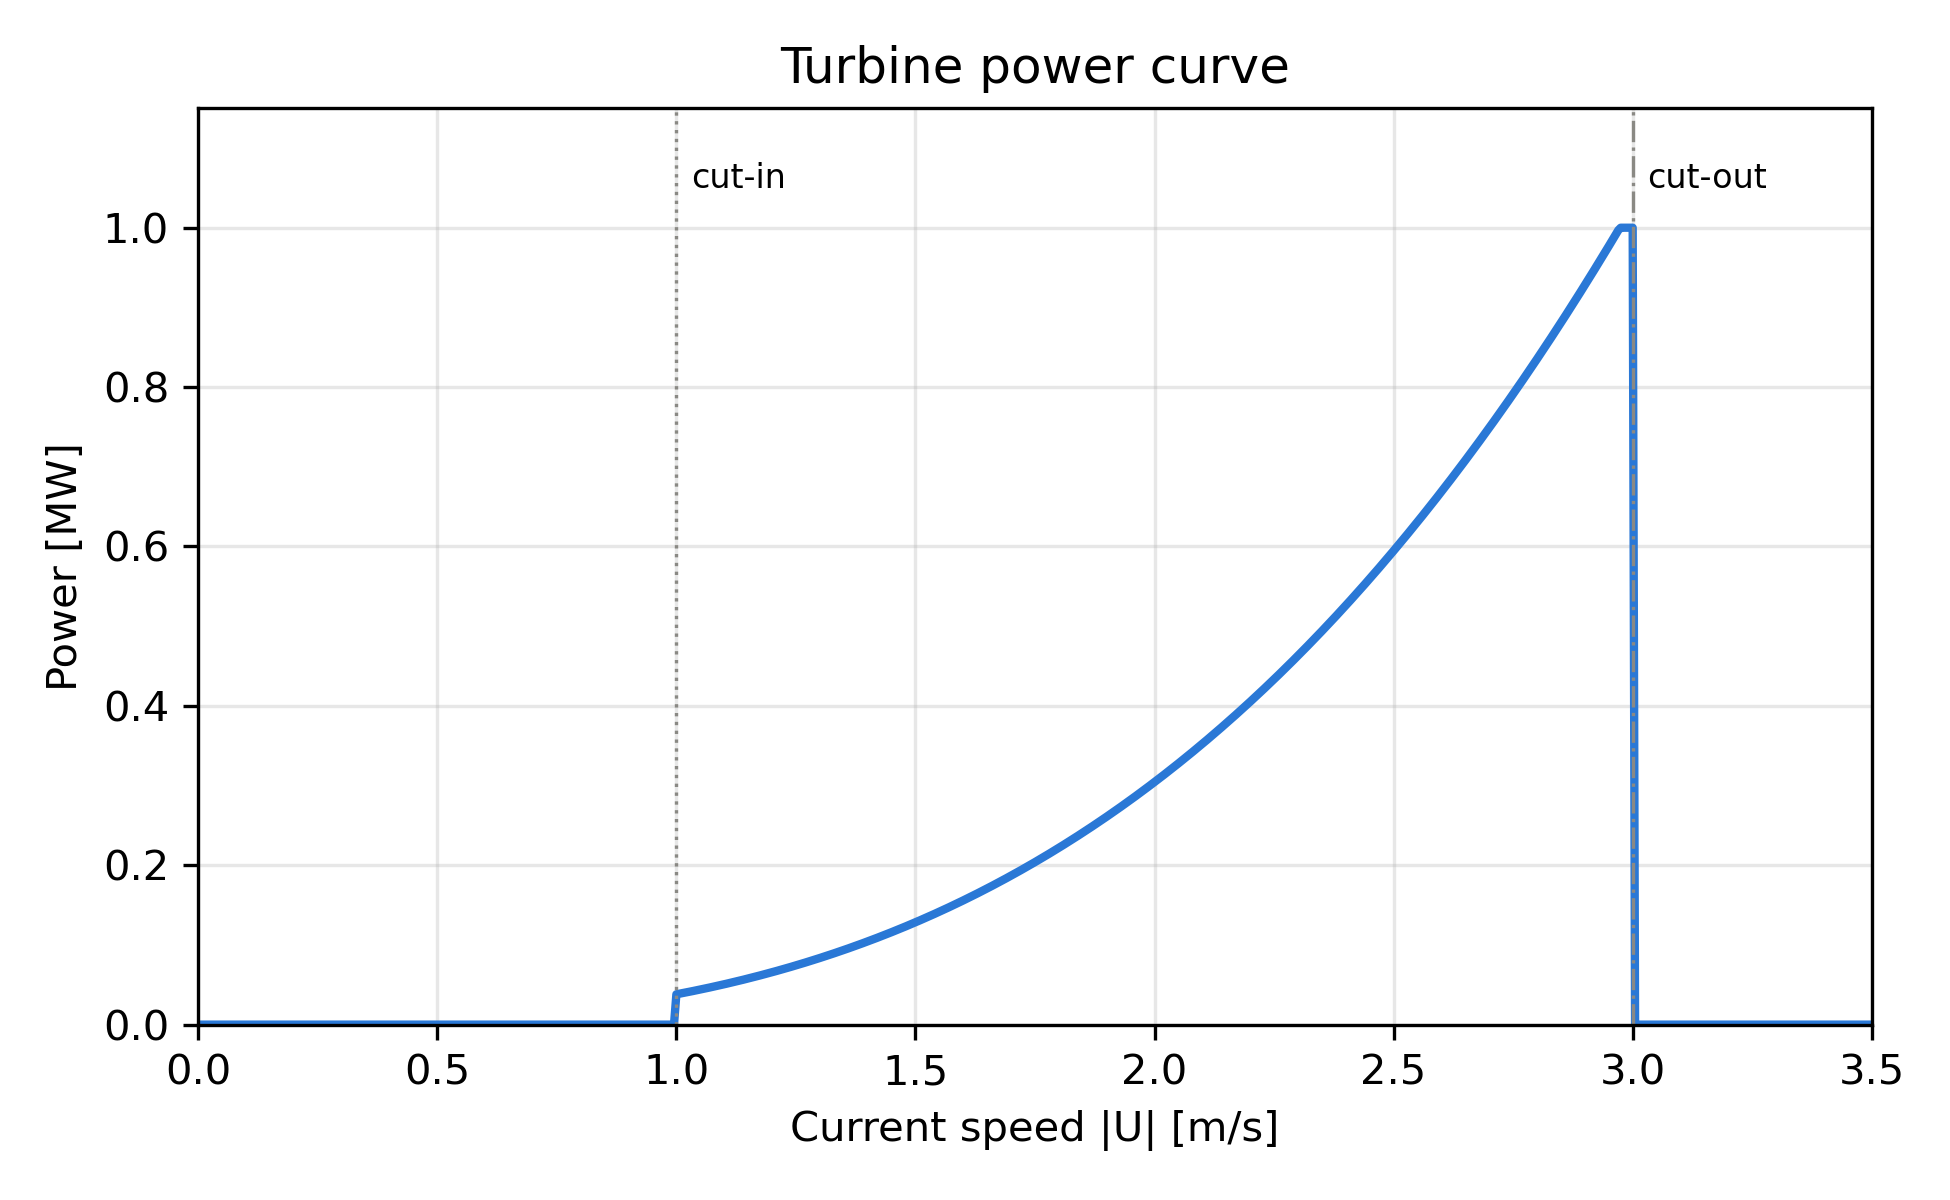
\includegraphics[width=0.7\textwidth]
    {figures/tidal/part2_tidal_power_curve.png}
    \caption{Power curve of the bi-directional hydrokinetic turbine.}
    \label{fig:stream-power-curve}
\end{figure}

\subsection{Power Production over 31 Days}
\label{sec:stream-power}
Applying Equation~\eqref{eq:stream-power} to the first 31 days of the reconstructed current gives the generated power shown in Figure~\ref{fig:stream-power-31days}. The turbine repeatedly saturates at its rated power of $1.0\,\mathrm{MW}$ around the strongest flood and ebb peaks, and drops to zero whenever the current falls below the $1.0\,\mathrm{m/s}$ cut-in, which occurs around every slack-water transition. The mean power over this 31-day window is $227.8\,\mathrm{kW}$.

\begin{figure}[H]
    \centering
    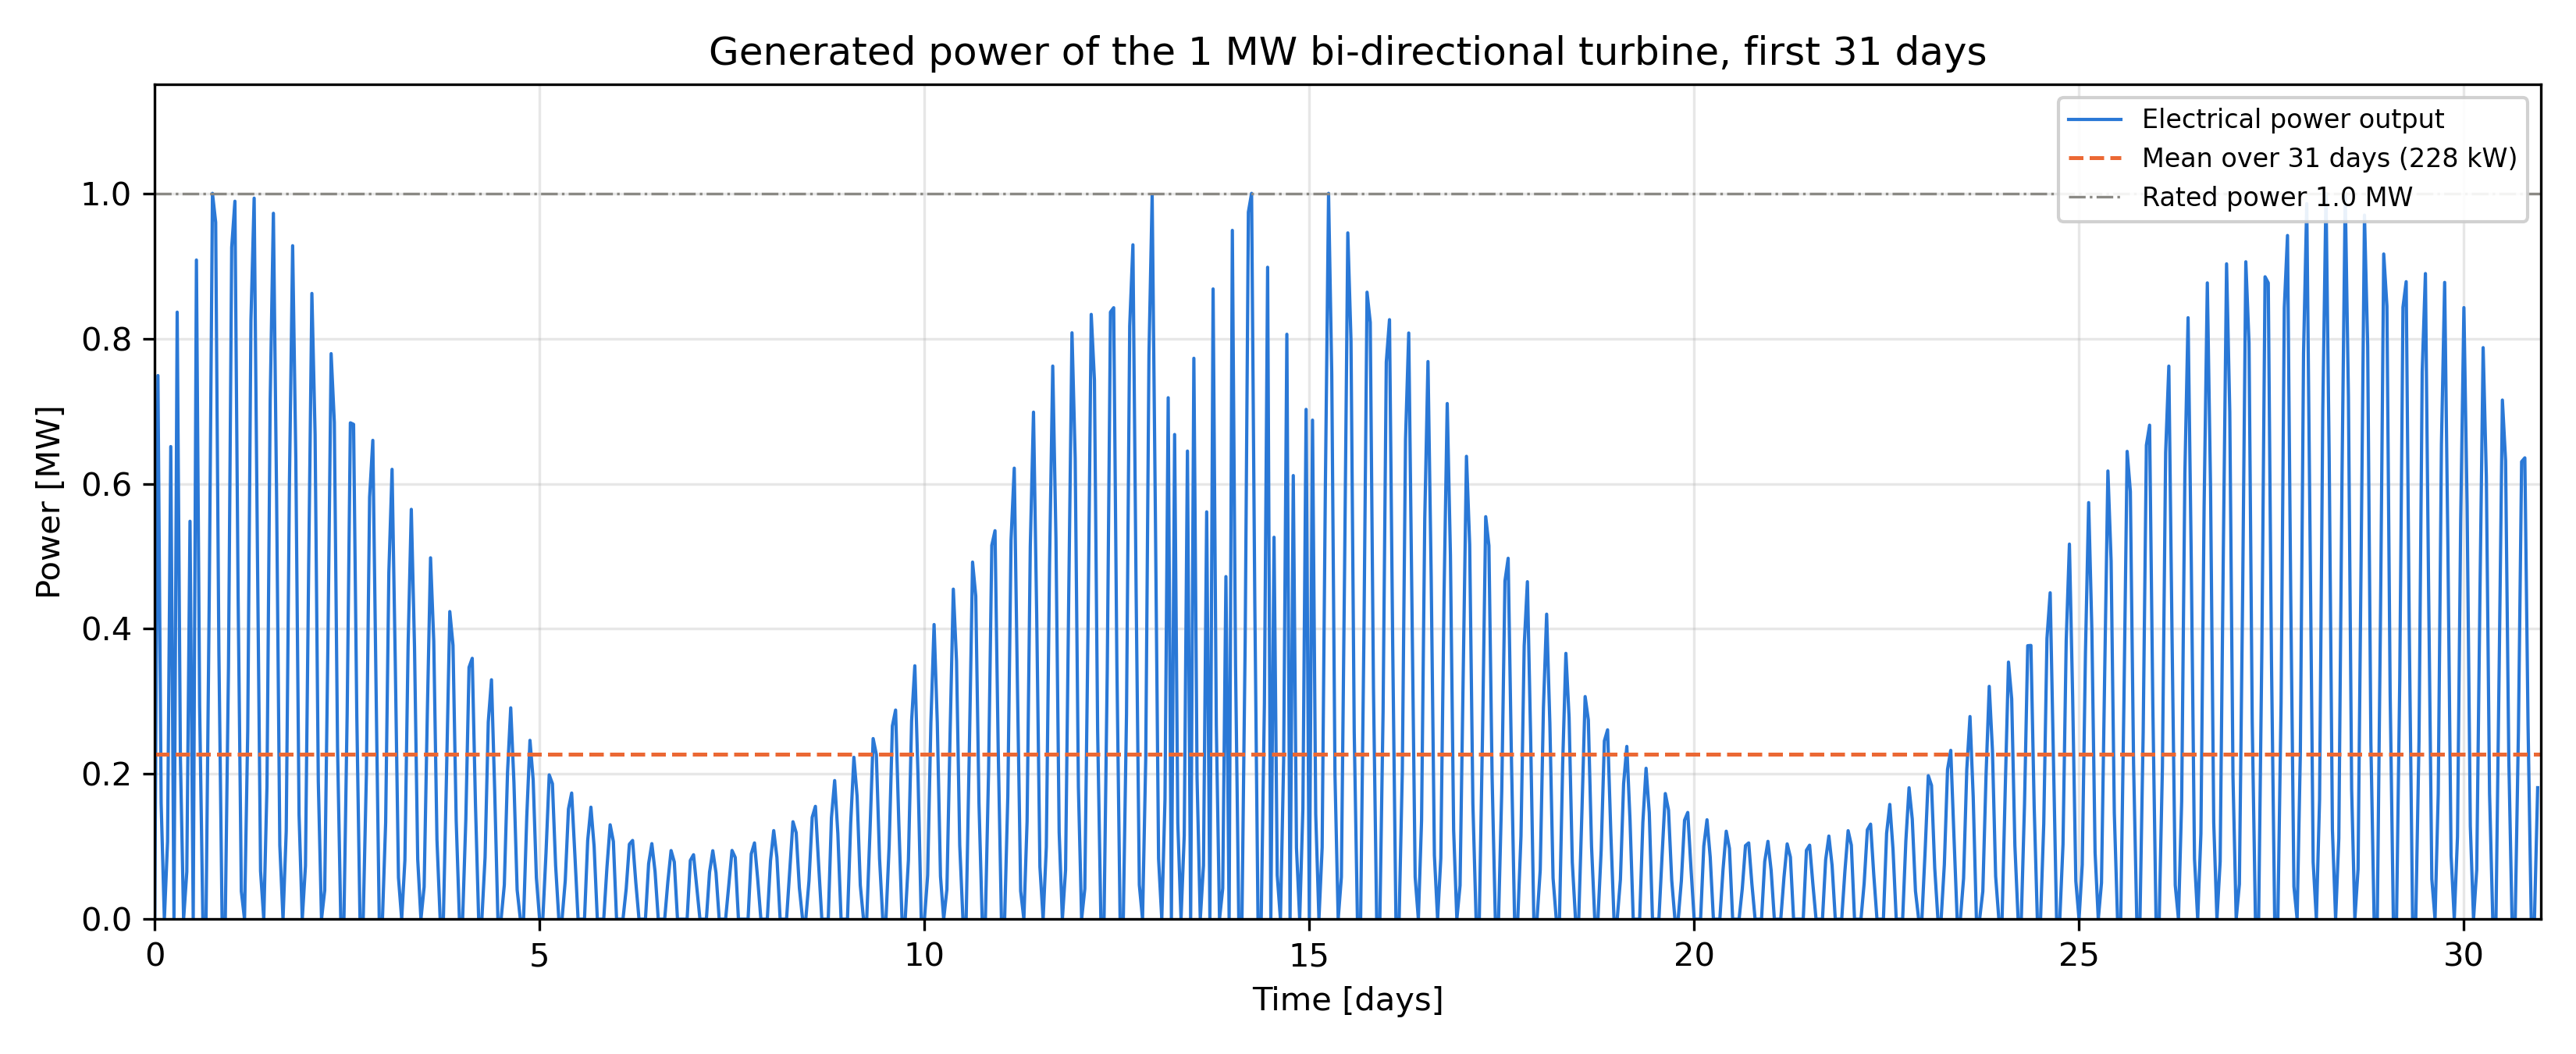
\includegraphics[width=\textwidth]
    {figures/tidal/part2_tidal_power_31days.png}
    \caption{Generated electrical power of the bi-directional turbine, first 31 days.}
    \label{fig:stream-power-31days}
\end{figure}

\subsection{Annual Mean and Maximum Power}
\label{sec:stream-annual-power}
Over the full year of $N=8760$ hourly values, the mean and maximum electrical power are

\begin{equation}
    \bar{P} = \frac{1}{N}\sum_{i=1}^{N} P_i, \qquad P_{max} = \max_i P_i,
    \label{eq:stream-meanmax}
\end{equation}

giving $\bar{P}=199.4\,\mathrm{kW}$ and $P_{max}$ equal to the rated power, $1000.0\,\mathrm{kW}$, which is reached for $22\,\mathrm{h}$ of the year. The turbine generates for $6012\,\mathrm{h}$ (68.6\,\% of the year); it is idle below cut-in for $2701\,\mathrm{h}$ (30.8\,\%) and above cut-out for $47\,\mathrm{h}$, the latter occurring during the strongest spring tides identified in Section~\ref{sec:tidal-cycle}.

\subsection{Annual Energy Yield and Capacity Factor}
\label{sec:stream-aey-cf}
The annual energy yield follows from summing the hourly power over the year,

\begin{equation}
    AEY = \sum_{i=1}^{8760} P_i\,\Delta t, \qquad \Delta t = 1\,\mathrm{h},
    \label{eq:stream-aey}
\end{equation}

giving $AEY = 1746.3\,\mathrm{MWh/yr} = 1.746\,\mathrm{GWh/yr}$. The capacity factor is

\begin{equation}
    CF = \frac{AEY}{P_{rated}\cdot 8760\,\mathrm{h}},
    \label{eq:stream-cf}
\end{equation}

which evaluates to $CF = 0.199 = 19.9\,\%$.

\subsection{Assumptions and Discussion}
\label{sec:stream-discussion}
Flood and ebb are treated as fully symmetric, with the turbine behaving as an ideal bi-directional device; the total efficiency of $0.45$ is held fixed over the whole operating range and availability is assumed to be $100\,\%$, so turbulence, rotor-plane shear, and wake and blockage effects between neighbouring devices are all neglected. The hourly time step also means that any short current peaks between samples are not captured when integrating energy.

The resulting capacity factor of approximately $20\,\%$ is low. This follows directly from the site's mean current speed of $1.44\,\mathrm{m/s}$ (Section~\ref{sec:tidal-cycle}), which is well below the $2.973\,\mathrm{m/s}$ rated speed of Equation~\eqref{eq:stream-rated}, combined with the current falling below cut-in for nearly a third of the year around slack water and during neap tides. A turbine with a lower rated speed -- through a larger capture area or a lower rated power -- would raise the capacity factor, at the cost of a lower peak output.

\section{Operation of a Tidal Range Power Plant}
\label{sec:tidal-range}

\subsection{Scheme, Input Data and Model Parameters}
\label{sec:range-inputs}
A tidal lagoon is formed with a $9\,\mathrm{km}$ wall enclosing a basin of approximately $10\,\mathrm{km^2}$, operated over an energy-generating lifetime of 120 years. The scheme consists of 10 bulb turbines of $20\,\mathrm{MWe}$ each, for a total installed capacity of $200\,\mathrm{MWe}$, and is operated as a one-way ebb-generation scheme: the basin is held near high water while the sea falls, generation starts once the head exceeds $H_{se}$ and stops once it falls below $H_{ee}$, after which the basin is refilled through sluices and the turbine passages without generating power. Table~\ref{tab:range-params} lists the scheme parameters used in the 0-D model.

\begin{table}[H]
    \centering
    \caption{Tidal range scheme and 0-D model parameters.}
    \label{tab:range-params}
    \begin{tabular}{lc}
        \hline
        Quantity & Value \\
        \hline
        Wall length / nominal basin area & $9\,\mathrm{km}$ / $\sim 10\,\mathrm{km^2}$ \\
        Turbines & $N=10$ bulb turbines $\times\, 20\,\mathrm{MWe} = 200\,\mathrm{MWe}$ \\
        Turbine diameter & $D = 8.0\,\mathrm{m}$ \\
        Turbine efficiency (fixed) & $\eta = 0.90$ \\
        Turbine flow rate (constant, all heads) & $Q_t = 500\,\mathrm{m^3/s}$ per turbine \\
        Sluice gate area & $500\,\mathrm{m^2}$ \\
        Discharge coefficient & $C_d = 1.0$ \\
        Start / end generating head & $H_{se}=3.0\,\mathrm{m}$, $H_{ee}=1.0\,\mathrm{m}$ \\
        Annual scaling factor (14-day cycle $\rightarrow$ year) & 24.377 \\
        \hline
    \end{tabular}
\end{table}

The basin area is not uniform, and instead depends on the basin water level $Z$ [m] as

\begin{equation}
    A(Z) = -264.55\,Z^4 - 3835.98\,Z^3 - 59920.6\,Z^2 + 554761.9\,Z + 1.1\times10^{7}\ \ [\mathrm{m^2}],
    \label{eq:range-area}
\end{equation}

which evaluates to $7.04$, $11.00$ and $11.63\,\mathrm{km^2}$ at $Z=-5$, $0$ and $+5\,\mathrm{m}$ respectively -- somewhat larger than the nominal $10\,\mathrm{km^2}$ over most of the operating range. The tidal elevation input is the supplied \texttt{Tidal\_range\_Dataset\_2026.csv}, containing 3360 samples at $\Delta t = 0.1\,\mathrm{h}$, covering a representative 14-day ($336\,\mathrm{h}$) spring-neap cycle with $Y$ ranging from $-4.99$ to $4.99\,\mathrm{m}$ about mean sea level.

\subsection{Zero-Dimensional Model and Operating Modes}
\label{sec:range-model}
The basin is represented as a single, uniform water level $Z(t)$, governed by the mass balance

\begin{equation}
    A(Z)\,\frac{dZ(t)}{dt} = Q(t),
    \label{eq:range-massbalance}
\end{equation}

discretised with a backward-difference scheme,

\begin{equation}
    Z_{i+1} = Z_i + \frac{Q_i}{A(Z_i)}\,\Delta t,
    \label{eq:range-update}
\end{equation}

with $\Delta t = 0.1\,\mathrm{h}$. The head difference is defined as $H(t) = Z(t) - Y(t)$, where $Y$ is the sea level; $H>0$ means the basin stands higher than the sea. The scheme cycles through four operating modes, summarised in Table~\ref{tab:range-modes}.

\begin{table}[H]
    \centering
    \caption{Operating modes of the one-way ebb-generation scheme.}
    \label{tab:range-modes}
    \small
    \begin{tabular}{lccc}
        \hline
        Mode & Condition to enter & Flow $Q$ (+ into basin) & Power \\
        \hline
        1. Filling (sluices + turbines open) & sea rises above basin, $H<0$ & $Q_s = C_d A_s\sqrt{2g|H|}$ & 0 \\
        2. Holding (after high water) & sea falls below basin, $H\ge 0$ & 0 & 0 \\
        3. Generating & $H \ge H_{se}$ & $-N Q_t$ & $P = N\rho g H Q_t \eta$ \\
        4. Holding (after generation) & $H < H_{ee}$ & 0 & 0 \\
        \hline
    \end{tabular}
\end{table}

$A_s$ is the total open area during filling: the sluice gates plus the 10 turbine passages, $A_s = A_{sluice} + N\pi D^2/4 = 500 + 502.7 = 1002.7\,\mathrm{m^2}$, since both sluices and turbines are opened to refill the basin. The initial basin level is set equal to the initial tidal elevation, $Z_0=Y_0$; since the supplied record starts at high water with the sea already falling, the model is initialised in the holding-after-high-water mode.

\subsection{Energy Potential during Spring and Neap Tides}
\label{sec:range-potential}
The water trapped at high tide has mass $\rho A R$ and a centre of gravity $R/2$ above low water, so the maximum energy available from a single tide of range $R$ over a constant basin area $A$ is

\begin{equation}
    E_{tide} = \frac{\rho g A R^2}{2}.
    \label{eq:range-potential}
\end{equation}

Averaged over one semi-diurnal tidal cycle of period $\tau \approx 12.42\,\mathrm{h}$, the corresponding mean power is

\begin{equation}
    \bar{P}_{TC} = \frac{\rho g A R^2}{2\tau}.
    \label{eq:range-meanpower}
\end{equation}

The largest and smallest high-water-to-low-water differences in the dataset give a spring range of $R_s = 9.92\,\mathrm{m}$ and a neap range of $R_n = 4.01\,\mathrm{m}$. Using the nominal basin area $A=10\,\mathrm{km^2}$ in Equations~\eqref{eq:range-potential}--\eqref{eq:range-meanpower}, this corresponds to $E_s = 1374\,\mathrm{MWh}$ per spring tide ($\bar{P}_{TC}=111\,\mathrm{MW}$) and $E_n = 224\,\mathrm{MWh}$ per neap tide ($18\,\mathrm{MW}$) -- a ratio of $(R_s/R_n)^2 \approx 6.1$.

As a check, the same potential is also computed accounting for the variable basin area of Equation~\eqref{eq:range-area}: the water lying between the low-water level $z_L$ and high-water level $z_H$ drops through a height $(z-z_L)$, so that

\begin{equation}
    E_{tide} = \rho g \int_{z_L}^{z_H} A(z)\,(z-z_L)\,dz,
    \label{eq:range-potential-var}
\end{equation}

which gives $1.553\,\mathrm{GWh}$ (spring) and $0.253\,\mathrm{GWh}$ (neap), about $13$--$15\,\%$ higher than the nominal-area estimate of Equation~\eqref{eq:range-potential}, consistent with the actual basin area exceeding $10\,\mathrm{km^2}$ through most of the operating range.

These values are theoretical upper bounds for a single ebb: the one-way scheme modelled in Section~\ref{sec:range-model} can only capture part of them, since generation cannot start until $H\ge H_{se}=3\,\mathrm{m}$, stops at $H=H_{ee}=1\,\mathrm{m}$, and the basin is never fully drained to low water.

\subsection{Basin Water Level and Head over 14 Days}
\label{sec:range-14days}
\begin{figure}[H]
    \centering
    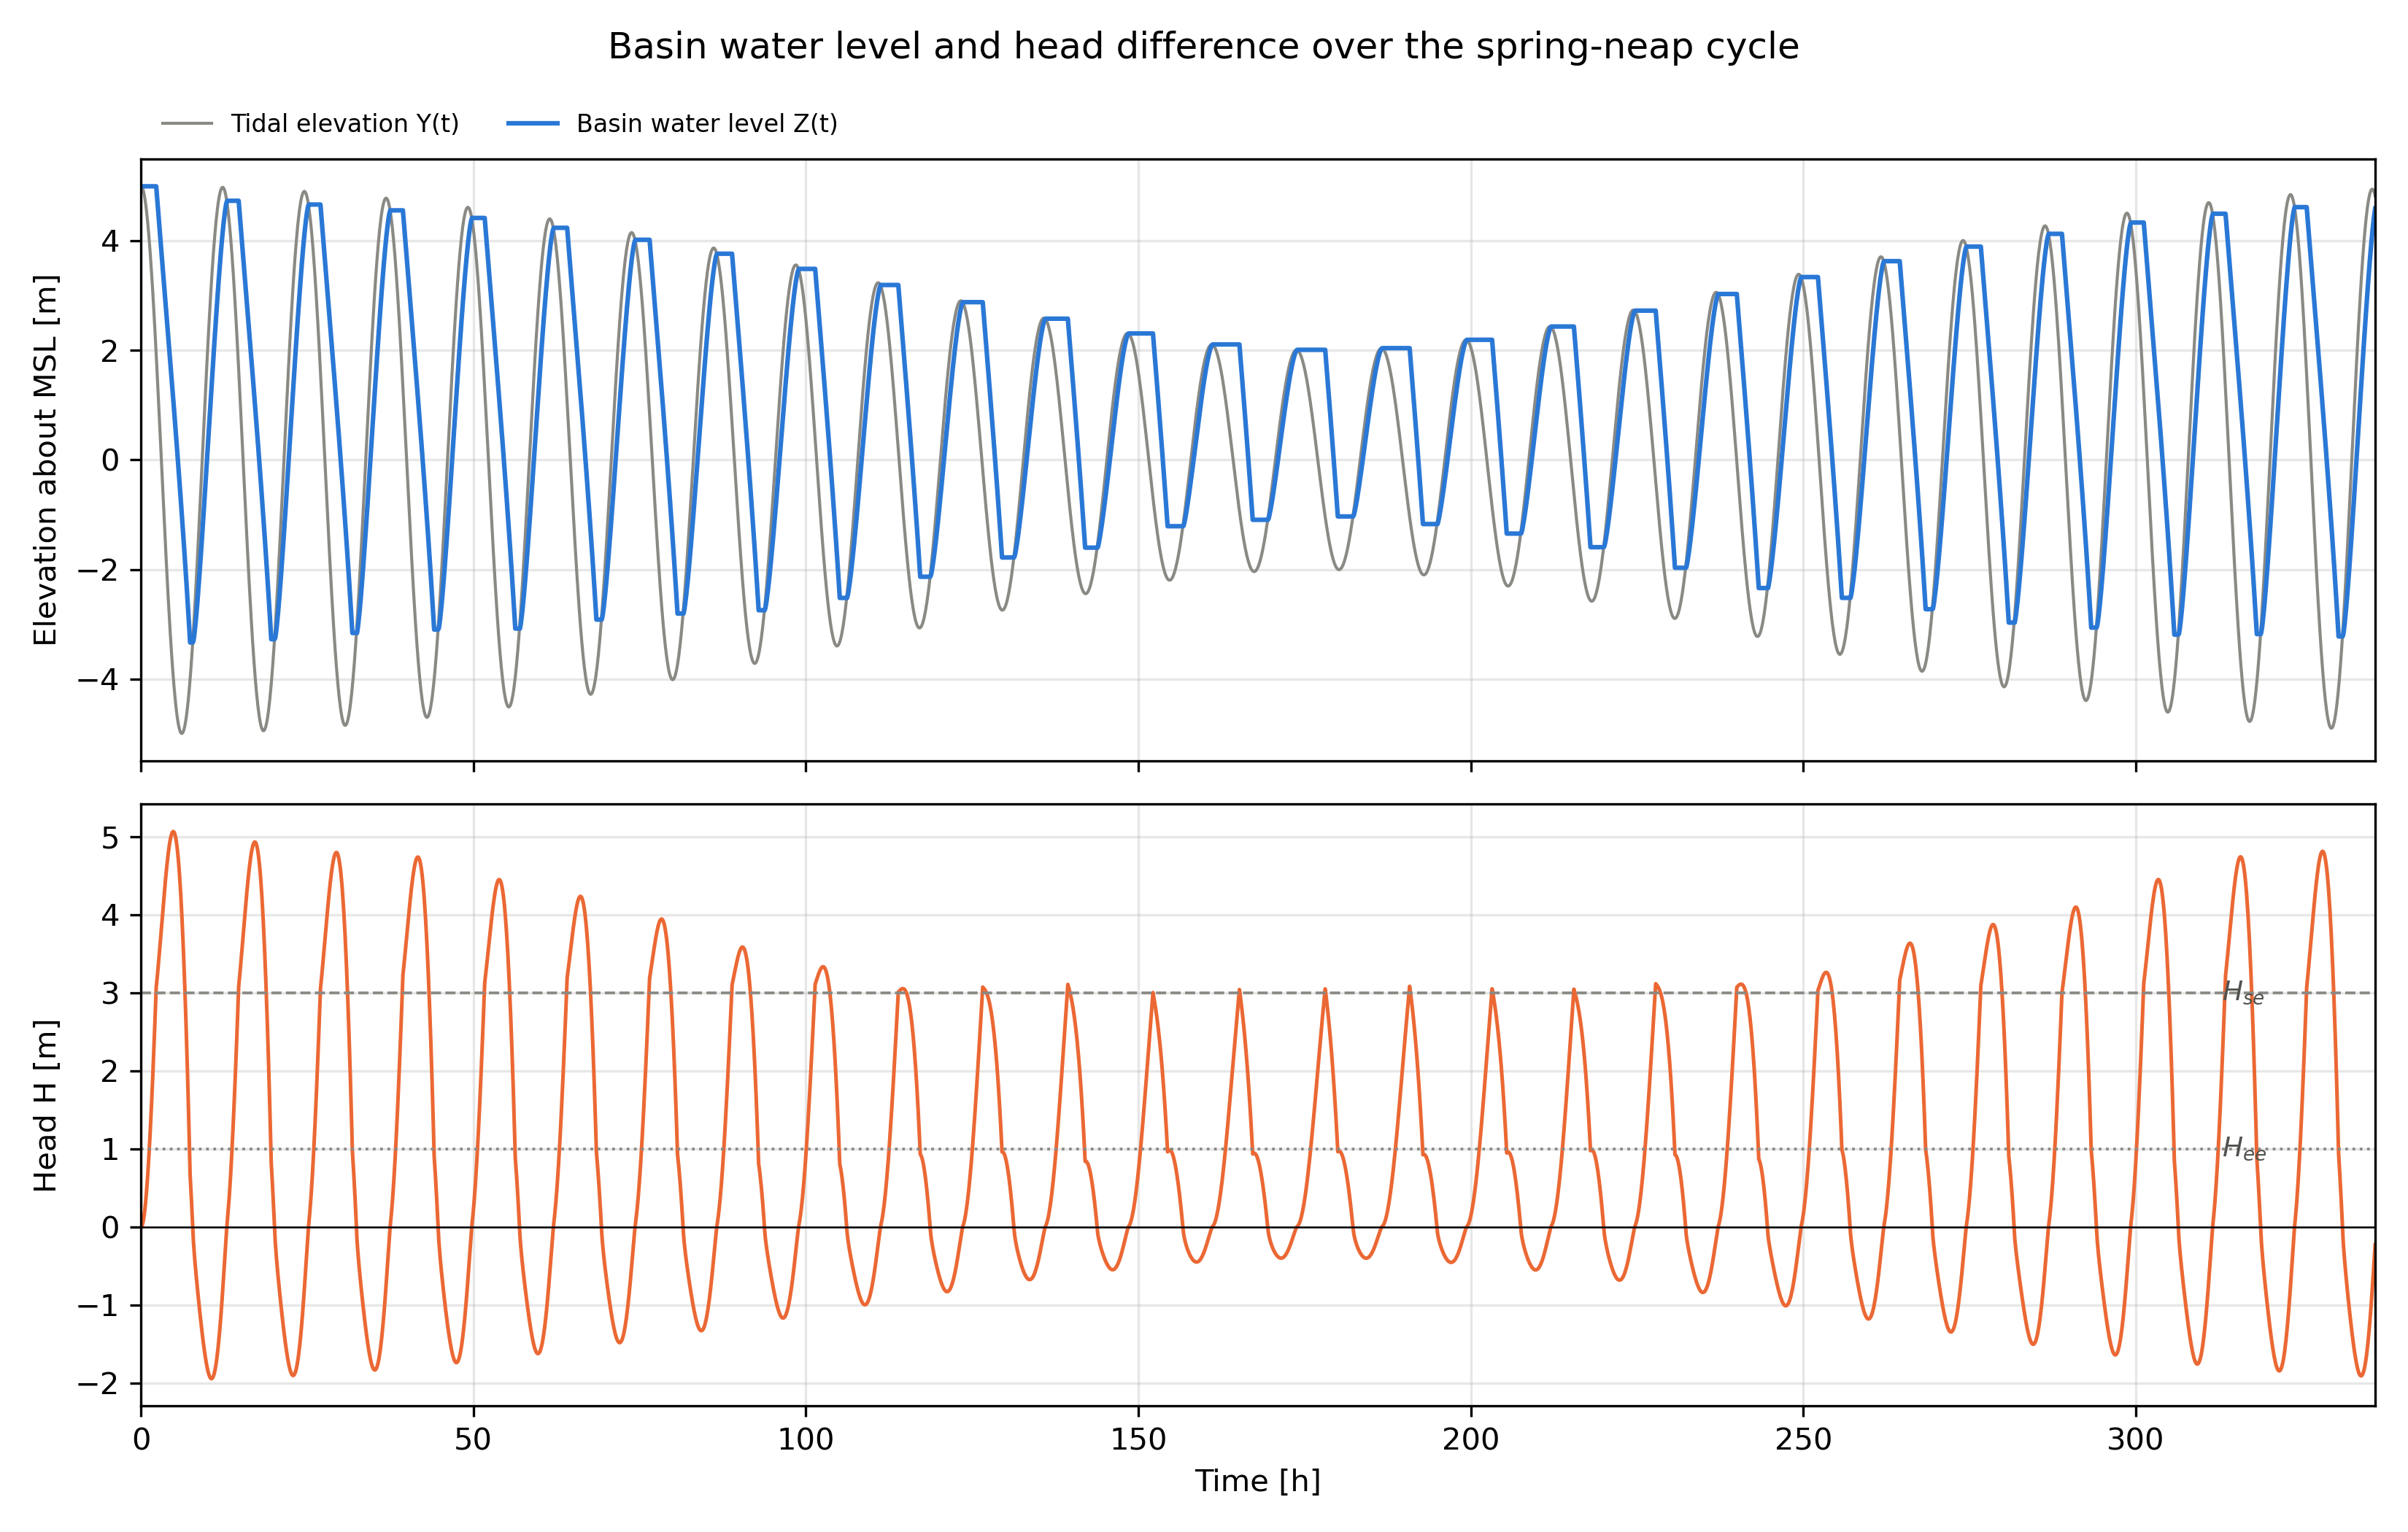
\includegraphics[width=\textwidth]
    {figures/tidal/part3_range_levels_head_14days.png}
    \caption{Basin water level and head difference over the 14-day spring-neap cycle.}
    \label{fig:range-14days}
\end{figure}
Figure~\ref{fig:range-14days} shows the basin following the sea upward during filling and then being held close to high water; it only falls again once the turbines start generating. During neap tides the sea falls less far below the held basin level, so the head barely exceeds $H_{se}$ and the resulting generating windows are noticeably shorter than during springs.

\subsection{Tidal Elevation, Basin Water Level and Operating Modes}
\label{sec:range-modes}
\begin{figure}[H]
    \centering
    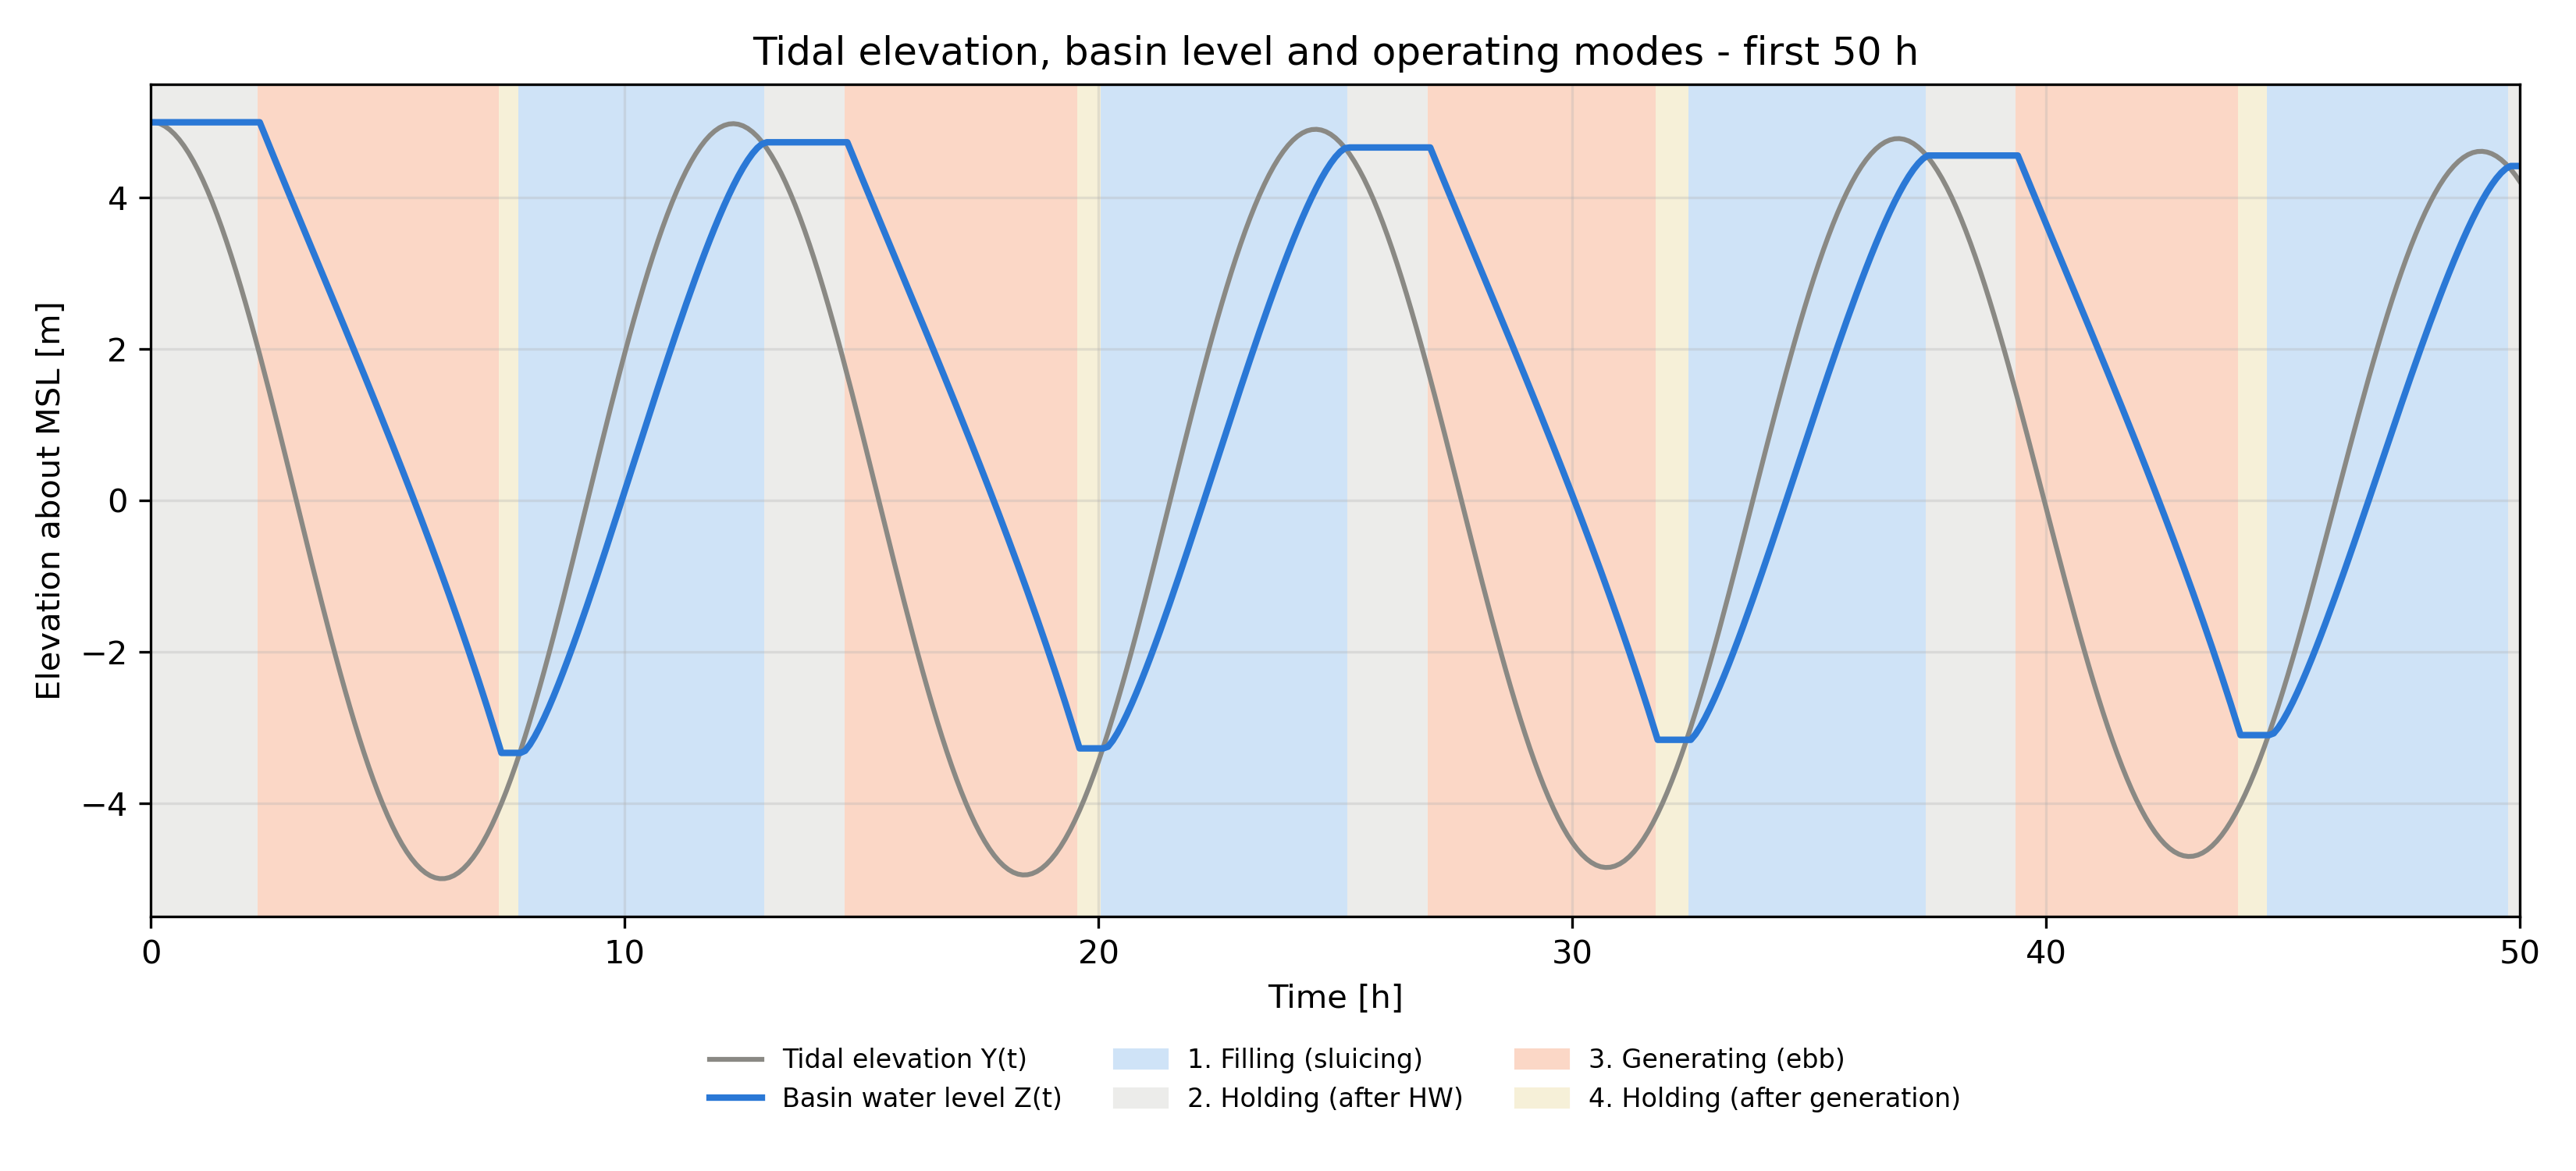
\includegraphics[width=\textwidth]
    {figures/tidal/part3_range_levels_modes_50h.png}
    \caption{Tidal elevation, basin water level and operating modes, first 50 hours.}
    \label{fig:range-modes-50h}
\end{figure}
Figure~\ref{fig:range-modes-50h} shows the tidal elevation and basin level over the first 50 hours, shaded by operating mode. Over the full 14-day record, filling accounts for $39.7\,\%$ of the time, holding after high water $21.0\,\%$, generating $29.3\,\%$ and holding after generation $10.0\,\%$, split over 27 separate generating periods. The maximum head reached during generation is $5.06\,\mathrm{m}$ (well above $H_{se}$, during the strongest spring tides), corresponding to a maximum electrical power of $229.2\,\mathrm{MW}$ -- above the $200\,\mathrm{MWe}$ installed capacity, a point returned to in Section~\ref{sec:range-discussion}.

\subsection{Hydraulic and Electrical Power}
\label{sec:range-power}
The total hydraulic power delivered to the turbines and the total electrical power produced are

\begin{equation}
    P_{hyd}(t) = N\rho g H(t) Q_t, \qquad P(t) = \eta\,P_{hyd}(t),
    \label{eq:range-power}
\end{equation}

shown for the first 50 hours in Figure~\ref{fig:range-power-50h}. Power is only produced while the scheme is in generating mode; it rises with the head as the basin drains and falls again as $H$ approaches $H_{ee}$, when the turbines shut down.

\begin{figure}[H]
    \centering
    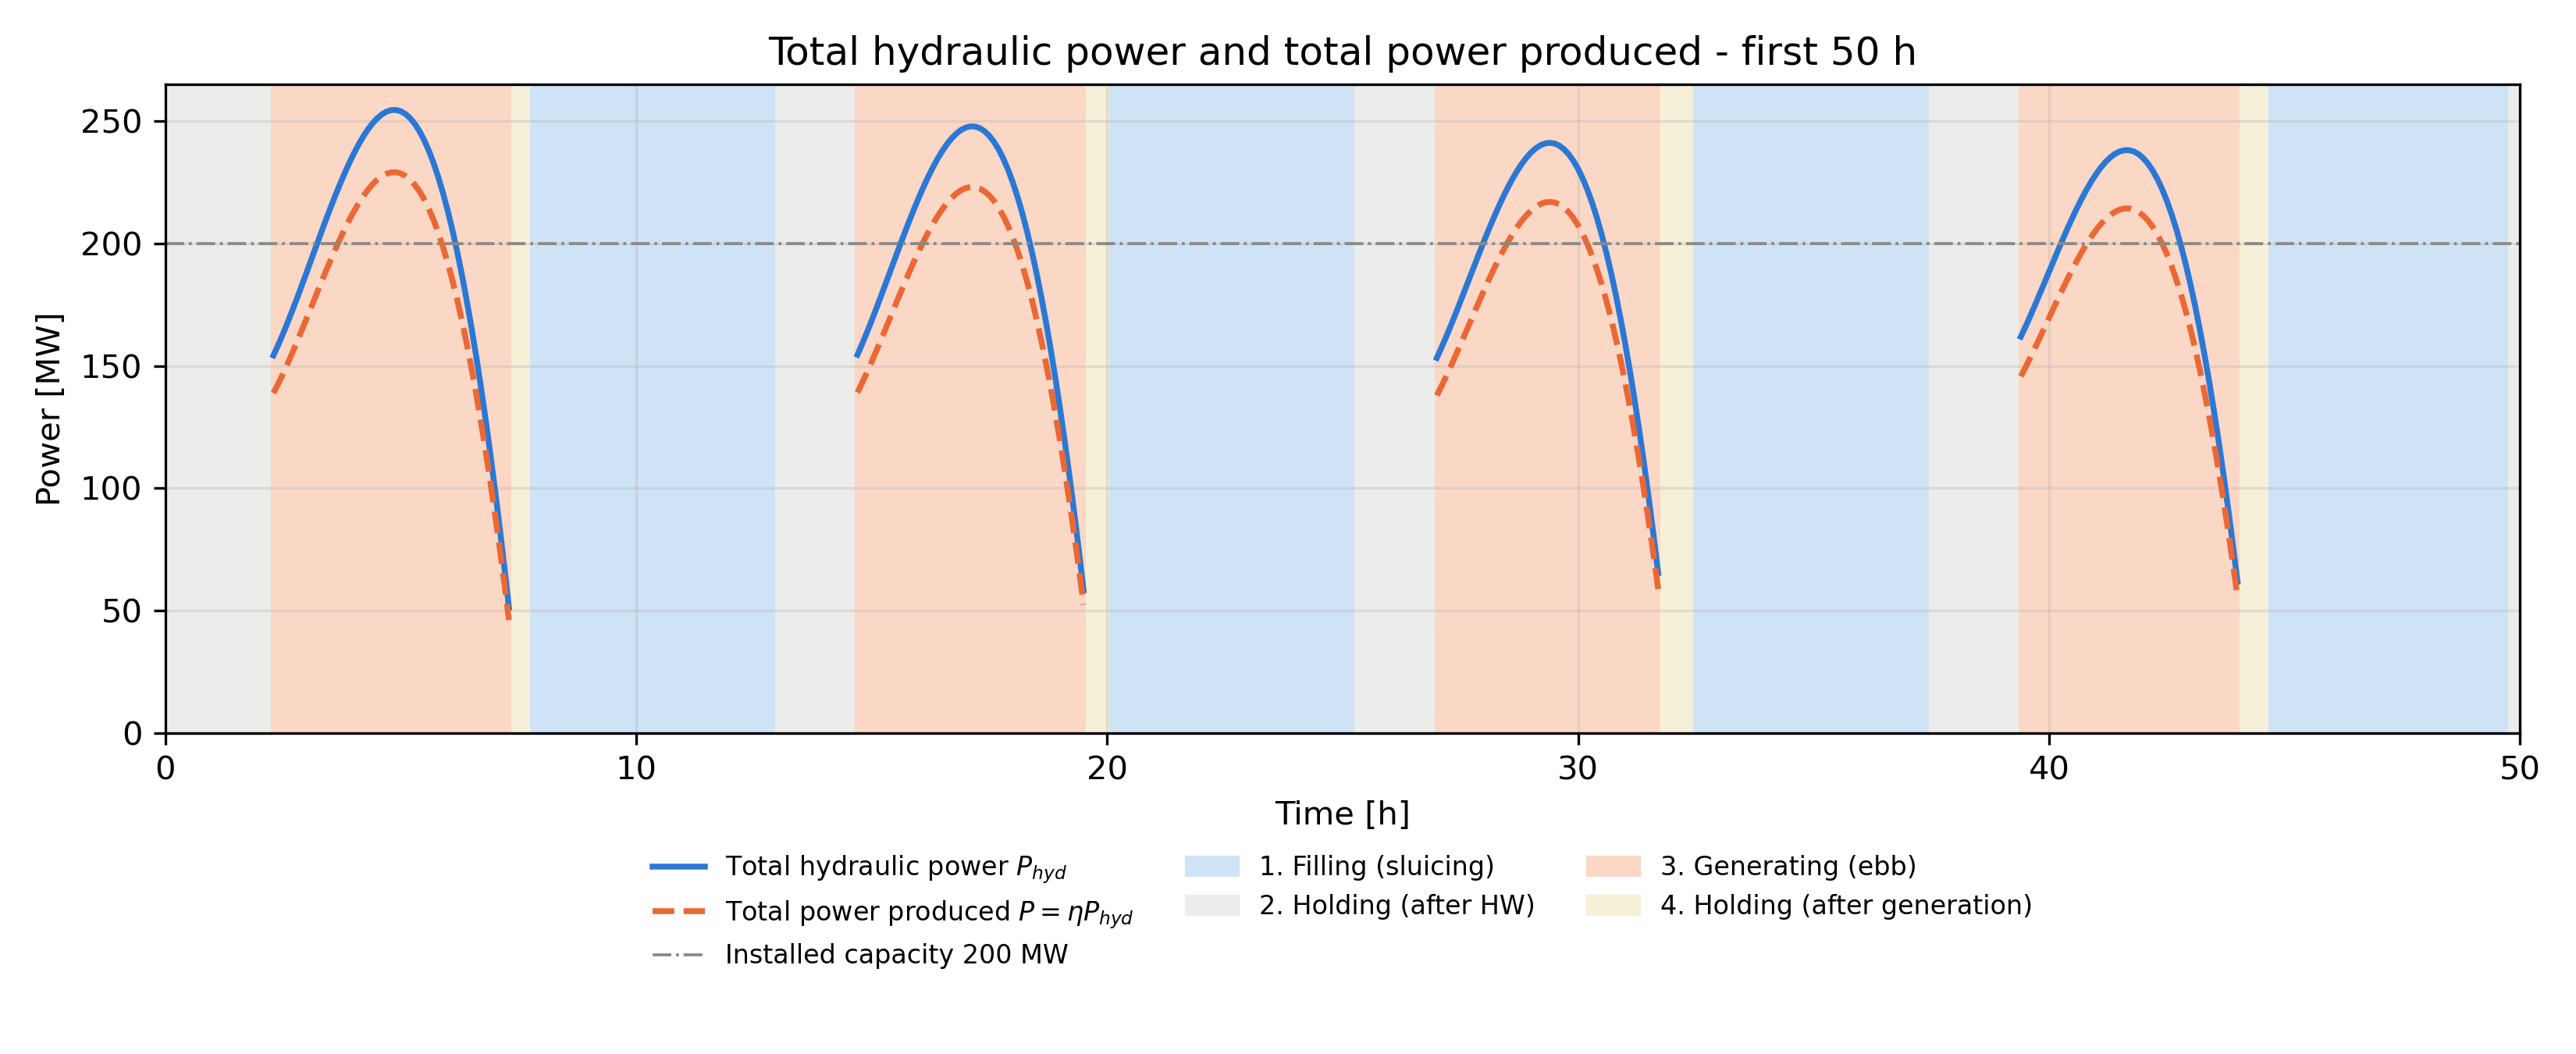
\includegraphics[width=\textwidth]
    {figures/tidal/part3_range_power_50h.png}
    \caption{Total hydraulic power and total electrical power produced, first 50 hours.}
    \label{fig:range-power-50h}
\end{figure}

\subsection{Total Flow Rates}
\label{sec:range-flow}
\begin{figure}[H]
    \centering
    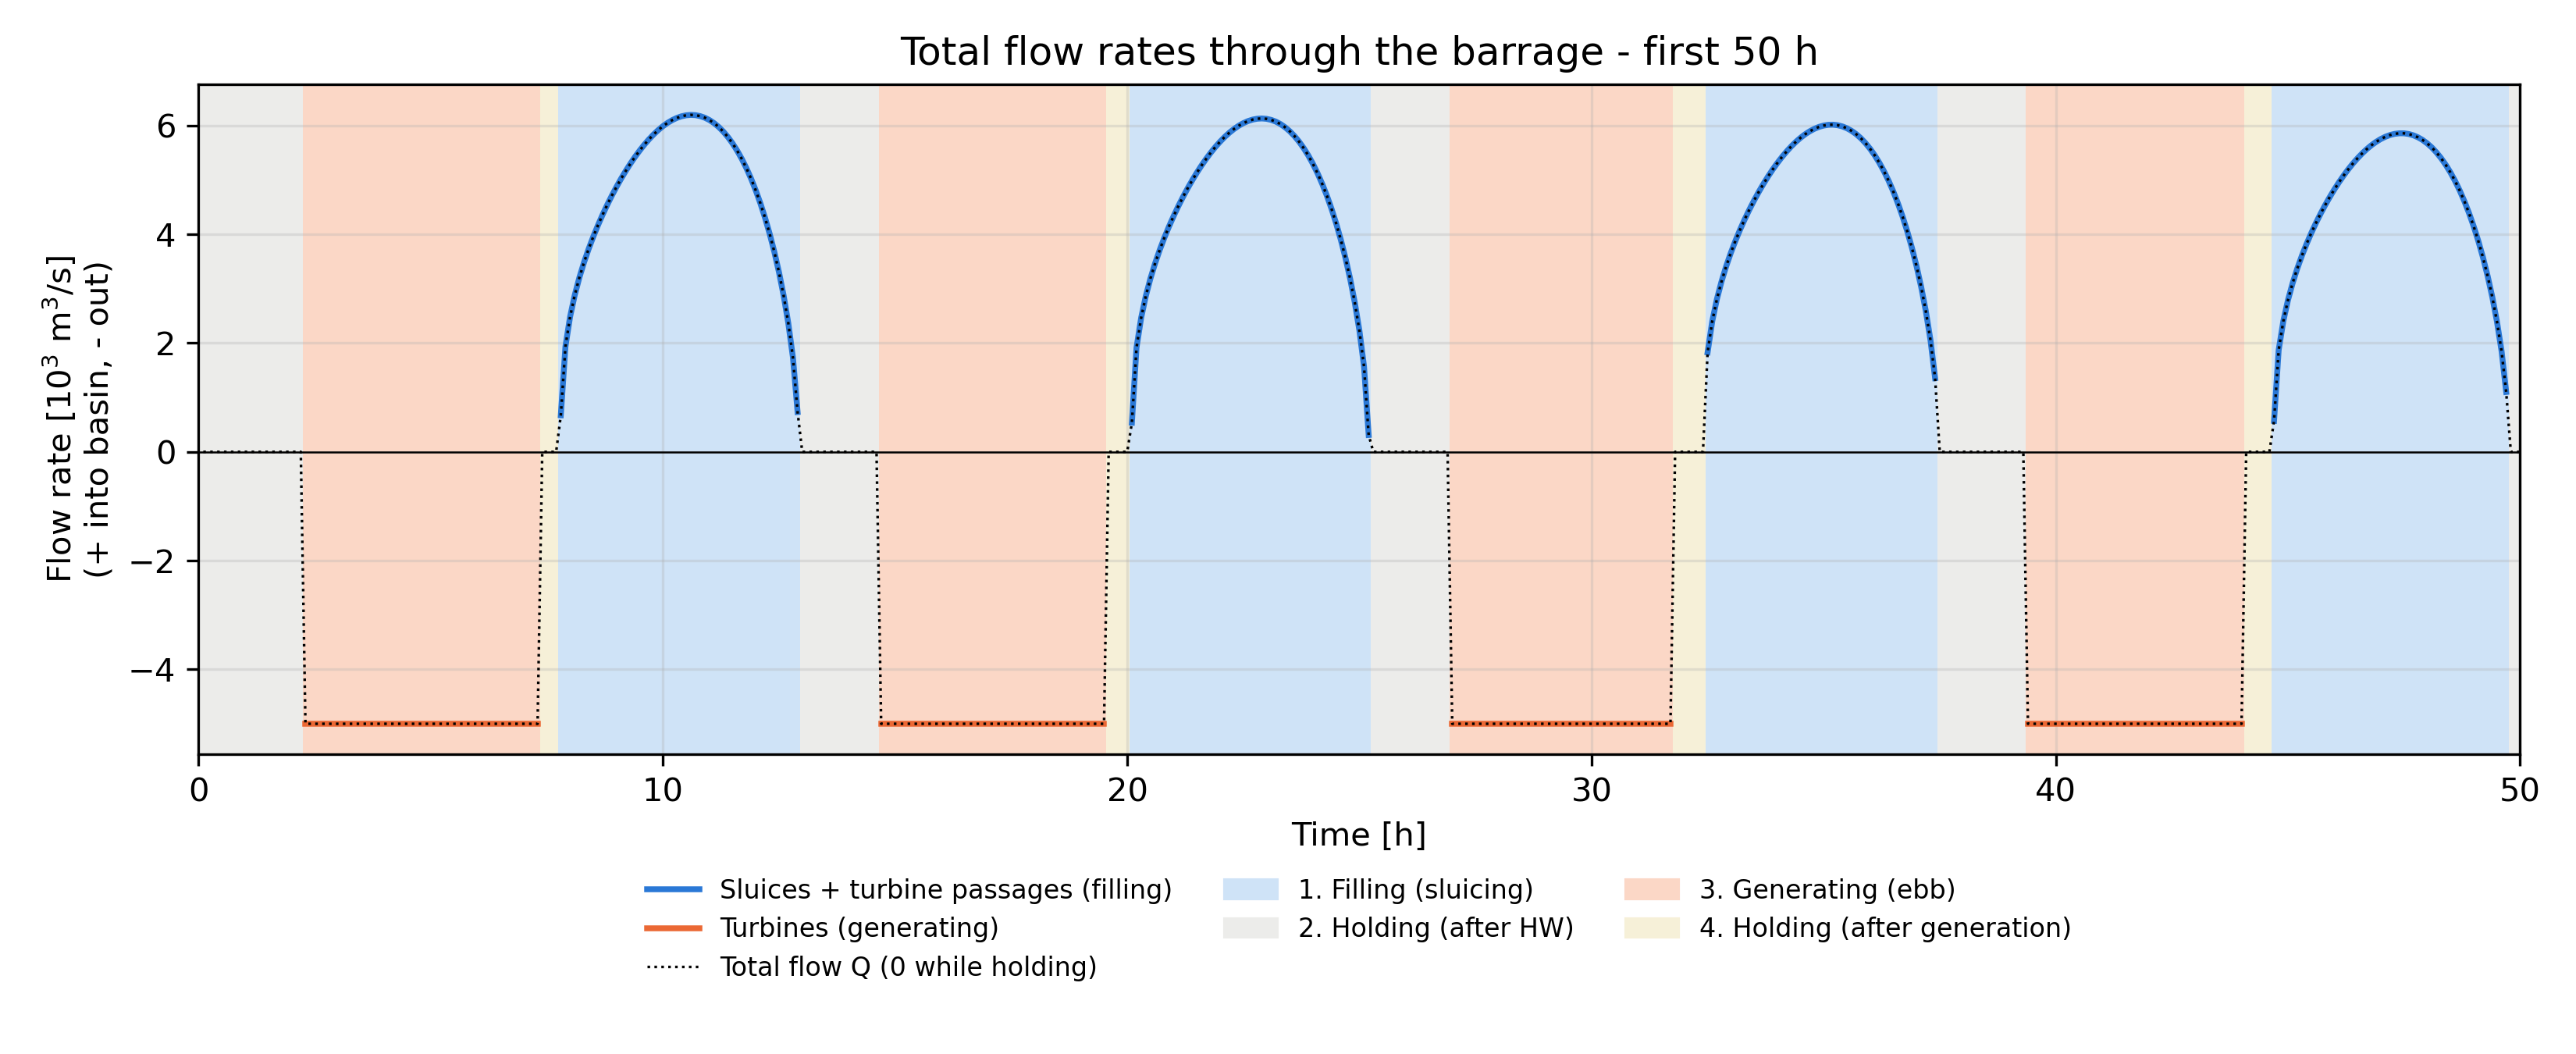
\includegraphics[width=\textwidth]
    {figures/tidal/part3_range_flow_50h.png}
    \caption{Total flow rates through the barrage, first 50 hours.}
    \label{fig:range-flow-50h}
\end{figure}
Figure~\ref{fig:range-flow-50h} uses the convention that positive flow enters the basin (filling through the sluices and turbine passages) and negative flow leaves through the turbines during generation. The flow is zero during both holding modes. The peak filling flow is $6195\,\mathrm{m^3/s}$, reached as the sea overtakes the held basin level at the largest heads; the flow through the turbines during generation is constant at $N Q_t = 5000\,\mathrm{m^3/s}$, by the model assumption of Table~\ref{tab:range-params}.

\subsection{Annual Energy Yield and Capacity Factor}
\label{sec:range-aey-cf}
Integrating the electrical power of Equation~\eqref{eq:range-power} over the 14-day record gives a cycle energy of $E_{14d} = 14.23\,\mathrm{GWh}$, of which $916\,\mathrm{MWh}$ is produced during the largest single spring ebb (67\,\% of the $1374\,\mathrm{MWh}$ potential of Section~\ref{sec:range-potential}) and $190\,\mathrm{MWh}$ during the smallest neap ebb (85\,\% of its $224\,\mathrm{MWh}$ potential); the mean power over the whole cycle is $42.4\,\mathrm{MW}$. Following Appendix 2, the 14-day record is taken as representative of the whole year, so that

\begin{equation}
    AEY = 24.377 \cdot E_{14d}, \qquad CF = \frac{AEY}{P_{installed}\cdot 8760\,\mathrm{h}},
    \label{eq:range-aey}
\end{equation}

giving $AEY = 346.9\,\mathrm{GWh/yr}$ and $CF = 0.198 = 19.8\,\%$.

\subsection{Assumptions and Discussion}
\label{sec:range-discussion}
The 0-D model represents the basin by a single, uniform, horizontal water level, and assumes that building the lagoon does not alter the tide on the seaward side of the barrage; filling is the only mode governed by the orifice equation, with $C_d=1$. The turbine flow rate $Q_t=500\,\mathrm{m^3/s}$ and efficiency $\eta=0.90$ are held fixed at every head, whereas a real bulb turbine follows a hill chart in which flow and efficiency fall off at low head and power is capped at the machine rating. This idealisation is visible in Section~\ref{sec:range-modes}: at the largest spring heads the model gives up to $229.2\,\mathrm{MW}$ total, exceeding the $200\,\mathrm{MWe}$ installed capacity. Capping the power at $200\,\mathrm{MWe}$ (time above rating occurs for $12.2\,\%$ of generating samples) reduces the estimate only slightly, to $AEY=343.4\,\mathrm{GWh/yr}$ ($1.0\,\%$ lower) and $CF=19.6\,\%$, since the exceedance is brief and confined to the very peak of the spring heads.

Switching between operating modes is assumed instantaneous, there is no pumping and no flood-generation, and the start/end generating heads $H_{se}$ and $H_{ee}$ are held fixed regardless of the tidal range; an optimised control strategy would adjust them tide by tide. Because the neap range of about $4\,\mathrm{m}$ only slightly exceeds $H_{se}=3\,\mathrm{m}$, neap tides leave only a short, low-head generating window and therefore contribute comparatively little to the annual yield, consistent with the $190\,\mathrm{MWh}$ neap-ebb energy against $916\,\mathrm{MWh}$ for the largest spring ebb. Finally, the supplied 14-day spring-neap cycle is assumed representative of the whole year (via the factor 24.377): seasonal and equinoctial variation of the tidal range, and the 18.6-year nodal cycle, are not captured, and $100\,\%$ availability is assumed throughout.
